\documentclass[]{article}

\usepackage[margin=1.0in]{geometry}
\usepackage{amsmath}
\usepackage{amsfonts}
\usepackage{amsthm}
\usepackage{graphicx}
\usepackage{amssymb}

\usepackage{mathtools}
\usepackage{caption}

%opening
\title{Finding Hausdorff Dimension of Limit Sets Using Spectral Theory}
\author{Alex Karlovitz}
\date{}

\begin{document}
	
	\maketitle

\section{A First Example}

We are interested in the Hecke group $\Gamma_R$ for $R > 0$ given by
\[
	\Gamma_R = \left\langle
	\begin{pmatrix}
		1 & R \\
		0 & 1
	\end{pmatrix},
	\begin{pmatrix}
		0 & -1 \\
		1 & 0
	\end{pmatrix}
	\right\rangle
\]
This of course corresponds to the maps $z \mapsto z + R$ and $z \mapsto -1/z$.
In particular, we will look at the case $R = 20/7$.
\\

It is straightforward to show that $\Gamma_{20/7}$ is conjugate to the group
\[
	\Gamma = \left\langle
	\begin{pmatrix}
		1 & 1 \\
		0 & 1
	\end{pmatrix},
	\begin{pmatrix}
		0 & -\frac{7}{20} \\
		\frac{20}{7} & 0
	\end{pmatrix}
	\right\rangle
\]
For our purposes, it is sufficient to consider $\Gamma$, since conjugation preserves the Hausdorff dimension of the limit set.
\\

In Figure \ref{fundDomain}, we see a fundamental domain for $\Gamma\backslash\mathbb{H}$.
\begin{figure}[h]
	\centering
	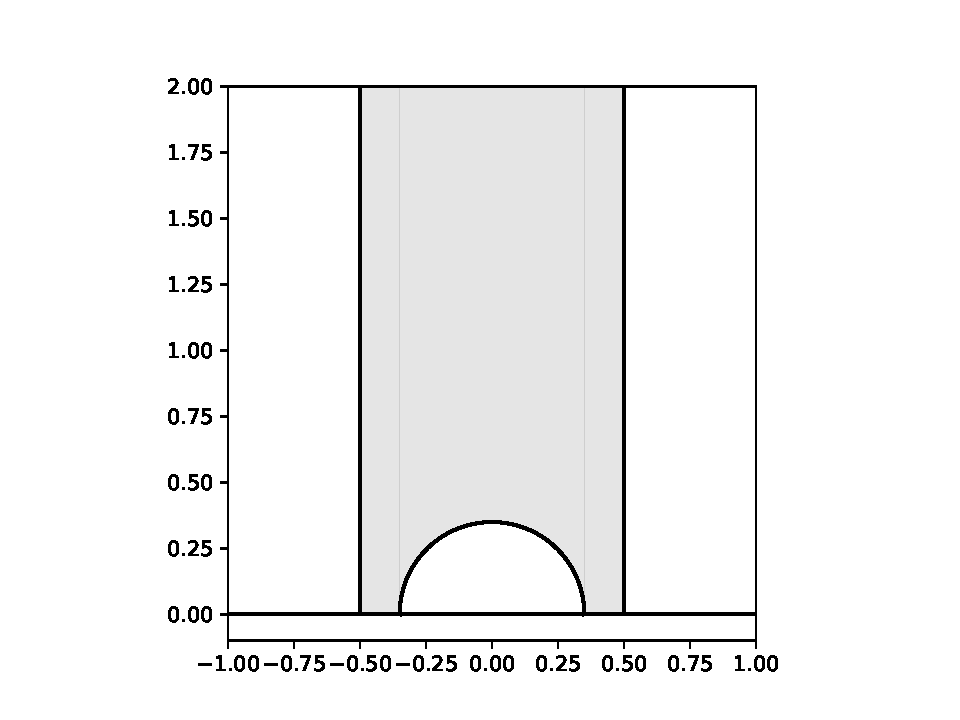
\includegraphics[trim = 75 20 80 35, clip, width=0.5\linewidth]{fundDomainGamma.pdf}
	\caption{Fundamental Domain for $\Gamma\backslash\mathbb{H}$}
	\label{fundDomain}
\end{figure}
This is clear because $z \mapsto z + 1$ gives the horizontal shift by 1, and $z \mapsto -R^2/z$ results in inversion through the circle of radius $R$.
Notice that this is an infinite volume fundamental domain, which is one way in which this case differs from the original $SL(2, \mathbb{Z})$ case.
\\

We are interested in finding the Hausdorff dimension $\delta$ of the limit set of $\Gamma\backslash\mathbb{H}$.
Patterson-Sullivan theory tells us that $\delta$ is related to the smallest eigenvalue $\lambda_0$ achieved by Maass cusp forms on $\Gamma$.
The relation is $\lambda_0 = \delta(1 - \delta)$.
So, we will compute $\delta$ by applying Hejhal's algorithm to $\Gamma$.
(One can even show that in the case of $\Gamma_R$ for $R \geq 2$, there is exactly one eigenvalue, and it falls between $0$ and $1/4$).
\\

Now let's discuss applying Hejhal's algorithm to $\Gamma$.
Suppose $f$ is a Maass cusp form for $\Gamma$.
(See notes from my learning seminar talk ``Maass Cusp Forms and Hejhal's Algorithm'' for more details).
Since
$
\begin{psmallmatrix}
1 & 1 \\
0 & 1
\end{psmallmatrix} \in \Gamma
$,
we have the same Fourier expansion as in the $SL(2, \mathbb{Z})$ case.
Thus, the same argument where we applied the Laplacian to the Fourier expansion applies here.
So we have that
$$
f(z) = a_0(y) + \sum_{n\neq0} a_n\sqrt{y}K_{\nu}(2\pi|n|y)e(nx)
$$
where $\nu \in \mathbb{C}$ is chosen so that $f$ is an eigenfunction of the Laplacian with eigenvalue $1/4 - \nu^2$.
The only difference in this case is that we are no longer working with a cusp form.
This is actually simpler than the non-constant terms case.
Since there is no $x$ in the constant term, the differential equation is
$$
\frac{1}{y^2}a_0''(y) - \lambda a_0(y) = 0
$$
where $\lambda = \delta(1 - \delta)$ and $\delta$ is chosen to be greater than $1/2$.
It is straightforward to see that the only two solutions are $y^\delta$ and $y^{1-\delta}$.
By the assumption that our Maass form is square-integrable around the cusp, we are able to throw out the $y^\delta$ term.
Hence,
$$
a_0(y) = a_0y^{1-\delta} = a_0y^{1/2 - \nu}
$$

It is straightforward to show (again, see the learning seminar talk) that $\nu = ir$ for $r > 0$ or $\nu \in \mathbb{R}$ with $|\nu| < 1/2$.
It turns out that in this case, there is indeed a real choice for $\nu$ in the spectrum.
\textbf{Why is this true?}
This is another way in which our current case will differ from the original $SL(2, \mathbb{Z})$ case.
\\

The only other way this case will differ from the $SL(2, \mathbb{Z})$ case is in the different fundamental domain.
To modify the existing code to fit this case, I will need to
\begin{itemize}
	\item Modify the $\mathcal{F}$-pullback function to work with $\Gamma\backslash\mathbb{H}$ instead of $SL(2, \mathbb{Z})\backslash\mathbb{H}$
	\item Make sure $K$-Bessel computations use subscript $\nu$, not just $ir$
	\item Add in the $a_0$ term
\end{itemize}

\subsection{Testing}

Let's discuss how we can test the code.
Kontorovich and Str\"ombergsson's result is that the Hausdorff dimension is
$$
\delta = 0.76705241700910205677150208864259506276668(7)
$$
The last digit is in parentheses to indicate that it may be off by $\pm1$.
This suggests that the smallest eigenvalue $\lambda_0 = \delta(1-\delta)$ has the following first 25 digits:
$$
\lambda_0 \approx 0.1786830065695966584789154
$$
Finally, recall that Hejhal's algorithm steps towards a value for $\nu$ where $\lambda_0 = 1/4 - \nu^2$.
Hence, we are actually looking for the value
$$
\nu \approx 0.26705241700910205677150208864259506276668(7)
$$
This is just $\nu = \delta - 1/2$.

\subsection{Results}

\textbf{June 27 2019}
I used the following parameters:
\begin{itemize}
	\item $D = 50$
	\item $M_0 = 30$
	\item $Q = 100$
	\item $Y_1 = 1/10$ and $Y_2 = 1/300$
\end{itemize}
I started with $\nu = 0.26$ and let the algorithm run.
Immediately, the program chose to step towards 0.19.
Since the true value starts out $\nu = 0.26...$, the code is not working as it should.
This is perhaps due to this method requiring a much higher degree of precision to observe the correct eigenvalue.
Another possibility is that $1/10$ is too high (meaning too many sample points are in the standard fundamental domain).
Of course, there is also a chance that there is an error in the code.
\\

I also checked what would happen if I changed $Y_1$ to $1/20$ and $M_0$ to $80$.
The same results were observed.
\\

\noindent \textbf{July 9 2019}
I tried using a higher precision with a larger number of Fourier coefficients to see if this would help.
I used the following parameters:
\begin{itemize}
	\item $D = 80$
	\item $M_0 = 80$
	\item $Q = 100$
	\item $Y_1 = 1/10$ and $Y_2 = 1/100$
\end{itemize}
This also stepped towards 0.19, interestingly.
However, this is still incorrect.
Perhaps an even higher precision...?

\section{A Disk Model Approach to the Same Problem}

Recall that we can map our work in the upper half plane to the unit disk via
$$
z \mapsto \frac{z - i}{z + i}
$$
(The inverse map is $\tau \mapsto i(1+\tau)/(1-\tau)$, where $\tau$ is taken in the unit disk).
Under this map, we can deduce the image of the fundamental domain from the previous section as follows.
First, notice that
$$
\pm\frac{1}{2} \mapsto -\frac{3}{5} \mp \frac{4}{5}i ~~~~~~~~~~
\pm\frac{7}{20} \mapsto -\frac{351}{449} \mp \frac{280}{449}i ~~~~~~~~~~
\infty \mapsto 1
$$
Next, since the geodesics in the disk model are circles normal to the unit circle, we can find the image of the geodesics from the upper half plane using these endpoints (see Figure \ref{fundDomainDisk}).
\begin{figure}[h]
	\centering
	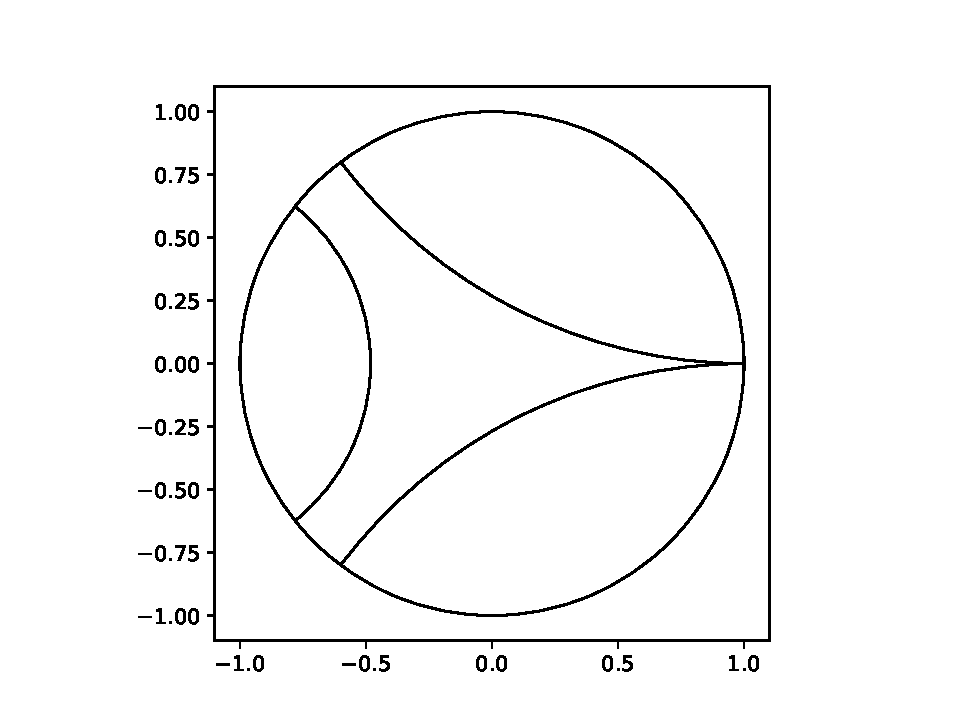
\includegraphics[trim = 75 20 80 35, clip, width=0.5\linewidth]{fundDomainDisk.pdf}
	\caption{Fundamental Domain in Disk Model}
	\label{fundDomainDisk}
\end{figure}

The new idea here is to apply Hejhal's algorithm to the fundamental domain in $\mathbb{D}$.
To do this, we begin by writing a Maass form $f$ in polar form $f(\rho, \theta)$.
Since $f$ is $2\pi$-periodic in $\theta$, it has a Fourier expansion
$$
f(\rho, \theta) = \sum_n a_n(\rho)\exp(in\theta)
$$
Next, since $f$ is a Maass form, it is an eigenfunction of the hyperbolic Laplace operator, say $\Delta f = s(1-s)f$.
After mapping to $\mathbb{D}$ and converting to polar coordinates, this operator is
$$
\Delta = \frac{(1 - \rho^2)^2}{4}\frac{\partial^2}{\partial\rho^2} +
\frac{(1 - \rho^2)^2}{4\rho}\frac{\partial}{\partial\rho} +
\frac{(1 - \rho^2)^2}{16\rho^2}\frac{\partial^2}{\partial\theta^2}
$$
Applying this map to the Fourier expansion, then using uniqueness of Fourier coefficients, we have that the $a_n(\rho)$'s satisfy the differential equation
$$
\frac{(1-\rho^2)^2}{4}a_n''(\rho) + \frac{(1-\rho^2)^2}{4\rho}a_n'(\rho) - \frac{n^2(1-\rho^2)^2}{16\rho^2}a_n(\rho) = s(1-s)a_n(\rho)
$$
As with the original case (where we worked in $\mathbb{H}$ and used the Fourier expansion at the cusp $\infty$), one finds that this differential equation has two solutions.
Only one of the solutions exhibits the appropriate decay, and hence we are able to deduce the form of the $a_n(\rho)$'s.
The result is that
$$
a_n(\rho) = a_n(1 - \rho^2)^2\rho^{|n|} \prescript{}{2}{F}_1(s, s+|n|, 1+|n|; \rho^2)
$$
where $\prescript{}{2}{F}_1$ is a hypergeometric function.
\\

To get a linear system, we first approximate $f$ by a finite Fourier expansion with $|n| \leq M$ (we are no longer assuming $f$ is a cusp form).
Then, we fix a distance $\rho = P$ from the origin and take $N \geq 2M+1$ equally spaced $\theta$'s to produce sample points.
For example, we could take the points $(P, \theta_j)$ where
$$
\theta_j = \frac{2\pi j}{N} ~~~~~\text{for}~~~~~0 \leq j < N
$$
We can then extract an expression for the Fourier coefficients by taking an appropriate linear combination of the function evaluated at the sample points.
This expression is
$$
a_n(P) = \frac{1}{N}\sum_{j=0}^{N-1}f(P, \theta_j)e^{-in\theta_j}
$$
Finally, we can set up a $(2M+1)\times (2M+1)$ linear system by using the $\Gamma$-automorphicity of $f$.
Let $(P_j^*, \theta_j^*)$ be the point in the chosen fundamental domain which is equivalent to $(P, \theta_j)$ mod $\Gamma$.
Some straightforward computation gives the following system
\begin{equation}\label{linSys}
	a_nc_n(P) = \sum_{|\ell| \leq M} a_\ell V_{n\ell}
\end{equation}
where
$$
c_n(\rho) = (1-\rho^2)^2\rho^{|n|} \prescript{}{2}{F}_1(s, s+|n|, 1+|n|; \rho^2)
~~~~~\text{and}~~~~~
V_{n\ell} = \frac{1}{N}\sum_{j=0}^{N-1}c_\ell(P_j^*)e^{i(\ell\theta_j^* - n\theta_j)}
$$
\textbf{Note}: recall that we set $s = 1/2 + \nu$ so that $\lambda = s(1-s) = 1/4 - \nu^2$.

\subsection{Results}

I plan to first test the disk method on $SL(2, \mathbb{Z})$ to make sure it is working correctly.
This, of course, is the Hecke group with parameter $R = 1$.
\\

\noindent \textbf{August 24 2019}

I tested the disk method on $SL(2, \mathbb{Z})$ with the following inputs:
\begin{itemize}
	\item $D = 50$
	\item $M_0 = 50$
	\item $N = 100$
	\item $\rho_1 = 9/10, \rho_2 = 49/50$
\end{itemize}
The final output was $9.619465$, which is incorrect.
The correct $r$-value near this is $9.53\dots$.
Perhaps we require higher precision...
\\

\noindent \textbf{August 27 2019}

I redid the test from August 24 with the following changes:
\begin{itemize}
	\item $D = 150$
	\item $M_0 = 100$
	\item $N = 250$
\end{itemize}
This also failed, as it found the value $8.9\dots$.
We will have to investigate what is causing this to fail.
One immediate thought is to print the values which go into the linear system and see if any of these are ``too large'' or ``too small.''
Perhaps this causes the numerics to be unstable.
\\

I ran another test today with the same $\rho_j$'s, but this time with
\begin{itemize}
	\item $D = 50$
	\item $M_0 = 50$
	\item $N = 101$
\end{itemize}
I printed out the values which are the pieces to build the linear system, and it appears the problem comes from the asymptotics of the hypergeometric function (See Section \ref{scaleSect} below).
I observed some values from the hypergeometric function as small as $10^{-60}$, while others were on the order of $10^{-3}$.
\\

\noindent \textbf{August 29 2019}

Today, I attempted to use the fix detailed in Section \ref{fix1} below.
The inputs were
\begin{itemize}
	\item $D = 50$
	\item $M_0 = 50$
	\item $N = 101$
	\item $\rho_1 = 1/2, \rho_2 = 1/3$
\end{itemize}
Surprisingly, this resulted in a ``matrix is numerically singular" error, even though this did not occur in the tests (described above) with larger $\rho$ values.
Inspecting the values of the hypergeometric function, I noticed some as small as $10^{-40}$.
These tiny values trickled into the linear system, where I saw entries as small as $10^{-20}$.
This, of course, is probably what caused the numerics to fail.
The question is: where are these tiny values coming from?

Another question is this: if I observed even tinier values when $\rho$ was closer to $1$, why didn't I get a ``matrix is numerically singular" error then?
This could simply be randomness, since the algorithm fails in both cases anyway.
\\

\noindent \textbf{September 3 2019}

Today, I attempted to use the fix detailed in Section \ref{fix2} below.
The inputs were
\begin{itemize}
	\item $D = 50$
	\item $M_0 = 50$
	\item $N = 101$
	\item $\rho_1 = 4999/1000, \rho_2 = 49/50$
\end{itemize}
And the matrix I used to map out of the standard fundamental domain was (the corresponding disk version of)
$$
A = T^{20}
$$
where $T$ is the shift map $z \mapsto z+1$.

The scaling worked beautifully here!
All the hypergeometric function values had norm close to $1$ (by ``close,'' I mean the norm was between $10^{-1}$ and $10$).
We still have the issue that the polynomial in $\rho$ that appears in the expression for $c_n$ can be very small.
I did notice values as small as $10^{-6}$ in the final linear system.

\textbf{Did it work?}

\subsection{Scaling the Hypergeometric Function}\label{scaleSect}

The linear system defined by Equation \ref{linSys} above could be given some fine-tuning before it can be run in the algorithm.
This is due to the hypergeometric function, which will be huge for some values of $s$ and $|n|$, and very tiny for others.
This leads to the matrix being ``numerically singular'' (that is, close enough to singular that Python gets confused).

One possible method of dealing with this is to scale the hypergeometric function by premultiplying by a function of $s$ and $|n|$.
The asymptotics of the function are derived here.
\\

Recall that the hypergeometric function $\prescript{}{2}{F}_1$ is defined
$$
\prescript{}{2}{F}_1(a, b, c; z) = \sum_{n=0}^{\infty}\frac{(a)_n(b)_n}{(c)_n}\frac{z^n}{n!}
$$
where $(q)_n$ is the Pochhammer symbol
\[
	(q)_n =
	\begin{cases}
		1 & n = 0 \\
		q(q+1)\cdots(q+n-1) & n \neq 0
	\end{cases}
\]
From this definition, we see that if $z \sim 0$, then $\prescript{}{2}{F}_1(a, b, c; z) \sim 1$.
\\

For our application, we will be using $z = \rho^2 \sim 1$.
To get an approximate size for the hypergeometric function near $z = 1$, we use the transformation formula
$$
\prescript{}{2}{F}_1(a, b, c; z) =
\frac{\Gamma(c)\Gamma(c-a-b)}{\Gamma(c-a)\Gamma(c-b)}\prescript{}{2}{F}_1(a, b, a+b+1-c; 1-z) $$$$ + \frac{\Gamma(c)\Gamma(a+b-c)}{\Gamma(a)\Gamma(b)}(1-z)^{c-a-b}\prescript{}{2}{F}_1(c-a, c-b, 1+c-a; 1-z)
$$
Since $\prescript{}{2}{F}_1(a, b, c; z) \sim 1$ when $z \sim 0$, this formula implies that
\begin{equation}\label{zSim1}
\prescript{}{2}{F}_1(a, b, c; z) \sim
\frac{\Gamma(c)\Gamma(c-a-b)}{\Gamma(c-a)\Gamma(c-b)} +
\frac{\Gamma(c)\Gamma(a+b-c)}{\Gamma(a)\Gamma(b)}(1-z)^{c-a-b} ~~~~~\text{when}~ z \sim 1
\end{equation}

Now let's move to our application.
Recall that we are interested in the function
$$
\prescript{}{2}{F}_1(s, s + |n|, 1 + |n|; \rho^2)
$$
where $s = 1/2 + \nu$ (given that $\lambda = 1/4 - \nu^2$ is the eigenvalue of a Maass form), $n \in \mathbb{Z}$ is bounded by $|n| \leq M$ ($M$ is how far we go out in the finite Fourier series approximation), and $\rho$ is the magnitude of $z$ (which we take to be near $1$).
If we plug these values into Equation \ref{zSim1}, we get
\begin{equation}\label{simApp}
\prescript{}{2}{F}_1(s, s + |n|, 1 + |n|; \rho^2) \sim
\frac{\Gamma(1 + |n|)\Gamma(1 - 2s)}{\Gamma(1 + |n| - s)\Gamma(1 - s)} +
\frac{\Gamma(1 + |n|)\Gamma(2s-1)}{\Gamma(s)\Gamma(s + |n|)}(1 - \rho^2)^{1 - 2s}
\end{equation}
for $\rho \sim 1$.
Next, we use Stirling's formula.
This is stated in Iwaniec-Kowalski as follows:
$$
\Gamma(s) = \left( \frac{2\pi}{s} \right)^{1/2}\left( \frac{s}{e} \right)^s\left( 1 + O\left( \frac{1}{|s|}\right) \right)
$$
This is valid in the sector $|\arg s| \leq \pi - \epsilon$ for any $\epsilon > 0$ (the implied constant depends on $\epsilon$).
Applying Stirling's formula to Equation \ref{simApp} gives
\begin{equation}\label{approxResult}
\prescript{}{2}{F}_1(s, s + |n|, 1 + |n|; \rho^2) \sim
\frac{(1+|n|)^{\frac{1}{2}+|n|}(1-2s)^{\frac{1}{2}-2s}}{(1+|n|-s)^{\frac{1}{2}+|n|-s}(1-s)^{\frac{1}{2}-s}} +
\frac{(1+|n|)^{\frac{1}{2}+|n|}(2s-1)^{2s-\frac{3}{2}}}{s^{s-\frac{1}{2}}(s+|n|)^{s+|n|-\frac{1}{2}}}(1-\rho^2)^{1-2s}
\end{equation}
I wrote code to test the accuracy of this statement, and it verified my claims.
\\

To finish, we wish to apply Equation \ref{approxResult} to our disk model approach.
Recall that a key step in deriving the linear system (\ref{linSys}) was removing the dependence of $a_n$ on $\rho$.
Hence, our scaling is not allowed to depend on $\rho$.
On the other hand, if we scale the $c_n(\rho)$'s with respect to $s$ and $n$, the $a_n$'s will be scaled accordingly.
This will \textit{not} break the derivation of Equation \ref{linSys}, and hence is a permissible scaling.

\subsection{Why Scaling May be in Vain}

If we take sample points at a fixed $\rho$ and with the $\theta_j$'s defined above, the $\mathcal{F}$-pullbacks could conceivably be anywhere in $\mathcal{F}$.
Since the Hecke groups always have a cusp, this means we can expect points with $\rho$ anywhere from $0$ to $1$.

For points with $\rho \sim 1$, we would like to use Equation \ref{approxResult} to scale.
For points with $\rho$ closer to $0$, we would like to use no scaling (since the Taylor expansion of the hypergeometric function suggests it will be close to $1$).
However, any choice of scaling must be used for \textit{all} points.

\section{First Idea to Fix Problems With Disk Method}\label{fix1}

The first idea we had to fix the problems described above is this: don't use $\rho$'s close to $1$.
In other words, choose the radii of the two circles on which we choose our sample points to be relatively small, say $\rho_1, \rho_2 \leq 1/2$.

Here are the pro's:
\begin{itemize}
	\item Since the Taylor series defining the hypergeometric function suggests that it is about $1$ when $\rho$ is close to $0$, we require no scaling.
	\item Not having to worry about scaling should fix the ``matrix is numerically singular" error.
	\item Given a point $z$ on the circle of radius $\rho$, its pullback $z^*$ to the standard fundamental domain for any Hecke group has $|z^*| \leq \rho$.
	See proof below.
\end{itemize}
And the con's:
\begin{itemize}
	\item Choosing $\rho$ values close to $1$ was done for a reason; specifically, this will cause the sample points to touch a large variety of fundamental domains.
	\item If too many sample points have neighboring sample points in the same fundamental domain, their pullbacks will too close together.
	\item These considerations may still result in a ``matrix is numerically singular" error (just for a different reason than before).
\end{itemize}

\subsection{Proof of Claim About Pullbacks from Circle}

First, recall that the M\"obius transformation which sends the disk model to the upper half plane model is
$$
z \mapsto i\frac{1 + z}{1 - z}
$$
One possible representative for this map in $SL(2, \mathbb{R})$ is
\[
	A =
	\begin{pmatrix}
		1 & 1 \\
		i & -i
	\end{pmatrix}
\]
Writing $S_\rho$ for the circle of radius $0<\rho<1$ centered at the origin, we are interested in the image $A(S_\rho)$ in the upper half plane.

We claim that $A(S_\rho)$ is the circle with center $i(1+\rho^2)/(1-\rho^2)$ and radius $2\rho/(1-\rho^2)$.
To see this, one may check that
\begin{itemize}
	\item $A(\rho) = i(1+\rho)/(1-\rho)$
	\item $A(-\rho) = i(1-\rho)/(1+\rho)$
	\item $i(1+\rho^2)/(1-\rho^2)$ is the midpoint of the two image points just described
	\item $A^{-1}(2\rho/(1-\rho^2) + i(1+\rho^2)/(1-\rho^2))$ has modulus equal to $\rho$
\end{itemize}
These facts, together with the fact that M\"obius transformations take circles to circles, imply that $A(S_\rho)$ is the circle we claimed it to be.

Next, for any $0 < \rho < \rho' < 1$, we have that the circle $A(S_\rho)$ is contained entirely within the interior of the disk whose boundary is $A(S_{\rho'})$.
Proving this is a straightforward computation.
Moreover, it is clear that the circles may described by a continuous function of $\rho$.
So the circles grow continuously as $\rho$ ranges from $0$ to $1$.

Finally, we conclude the proof by showing that the pullback of every point on $A(S_\rho)$ to the standard fundamental domain is in the interior of the disk whose boundary is $A(S_\rho)$.
This will finish the proof by the previous paragraph.

\textbf{SHOW THIS!!!}

\subsection{Results}

\textbf{9/21/2019}

Running this method with both $\rho = 1/2$ and $\rho = 1/3$ still resulted in a ``matrix is numerically singular" error.
However, after inspecting the matrices involved, it appears that the issue is still a scaling issue.
Specifically, some of the matrix entries are still very tiny while others are still very huge.

\textbf{I will need to look into this.}

\section{Second Idea to Fix Problems With Disk Method}\label{fix2}

Another idea to fix the issues described above is this: replace the standard fundamental domain with another one.
In particular, perhaps we could take a fundamental domain which is contained entirely outside of the closed disk of radius $\rho$ for some $\rho$ ``close'' to $1$.

Here are the pros of this approach:
\begin{itemize}
	\item We can return to using $\rho$ values close to $1$ for the sample points.
	\item Since all $\rho$ values involved will be close to $1$, we can use the scaling of the hypergeometric function introduced in Equation \ref{approxResult}.
	\item Since all points will be using an appropriate scaling, perhaps this will fix the ``matrix is numerically singular" error.
\end{itemize}
And the cons:
\begin{itemize}
	\item Although all fundamental domains have the same hyperbolic area, this choice of fundamental domain will have a small Euclidean area.
	\item The hypergeometric function is continuous in each of its entries, so the lack of variety in $\rho$ values could result in a lack of information, again causing a ``matrix is numerically singular" error.
\end{itemize}
	
\end{document}